% A skeleton file for producing Computer Engineering reports
% https://kgcoe-git.rit.edu/jgm6496/KGCOEReport_template

\documentclass[CMPE]{../KGCOEReport}

% The following should be changed to represent your personal information
\newcommand{\classCode}{CMPE 460}  % 4 char code with number
\newcommand{\name}{Andrei Tumbar}
\newcommand{\LabSectionNum}{1}
\newcommand{\LabInstructor}{Beato}
\newcommand{\TAs}{Xavier Brooks\\
Diana Yakobchuk}
\newcommand{\exerciseNumber}{1}
\newcommand{\exerciseDescription}{Intro to MSP432}
\newcommand{\dateDone}{1/14/2022}

\usepackage{tikz}
\usepackage{circuitikz}
\usetikzlibrary{calc}
\usepackage{multirow}
\usepackage{titlesec}
\usepackage{float}
\usepackage{lmodern}
\usepackage{pgfplots}
\usepackage{siunitx}
\usepackage{subcaption}
\usepackage{graphicx}
\usepackage[usestackEOL]{stackengine}
\usepackage{scalerel}
\usepackage[T1]{fontenc}
\usepackage{amsmath}
\usepackage{pdfpages}


\def\code#1{\texttt{#1}}

\begin{document}
    \maketitle
    \section*{Description}

    The focus of this laboratory exercise was to introduce the basics of operating the
    MSP432 development board as well as familarize students with GPIO pin operation.
    LEDs were controlled as GPIO pin outputs controlled from switches on the board.

	\subsection*{GPIO Commands}

	Each register below will control the settings for multiple pins on a single port.
	Most ports contain 8 pins each of which can be selected by the bit number on that register. For example, \code{BIT3} will select pin 3.

	\begin{enumerate}
  \item{\code{P1->SEL0}, \code{P1->SEL1}:}
  Two bits that select the functionality of the pin in question. \code{00}: General purpose IO. \code{01} Primary function, \code{10} Secondary function, \code{11} Tertiary function. Primary, secondary, and tertiary function will vary based on the specific pin in question.
  \item{\code{P1->DIR}:}
  Selects the direction of the pin IO. \code{0} input direction, \code{1} output direction.
  \item{\code{P1->DS}:}
  Selects the drive strength of the pin if the pin supports high drive strength. \code{0} regular drive strength, \code{1} high drive strength.
  \item{\code{P1->OUT}:}
  When the pin is configured as an output, this bit will control the output value. On input mode it will control if the bit is being pulled down (\code{0}) or pulled up (\code{1}) by a pull-up or pull-down resistor.
  \item{\code{P1->REN}:}
  Selects whether or not the pull-up/pull-down resistors should be enabled. Only useful when pin is in input mode. Disabling this bit will cause the \code{OUT} bit value on this pin to be ignored.
\end{enumerate}

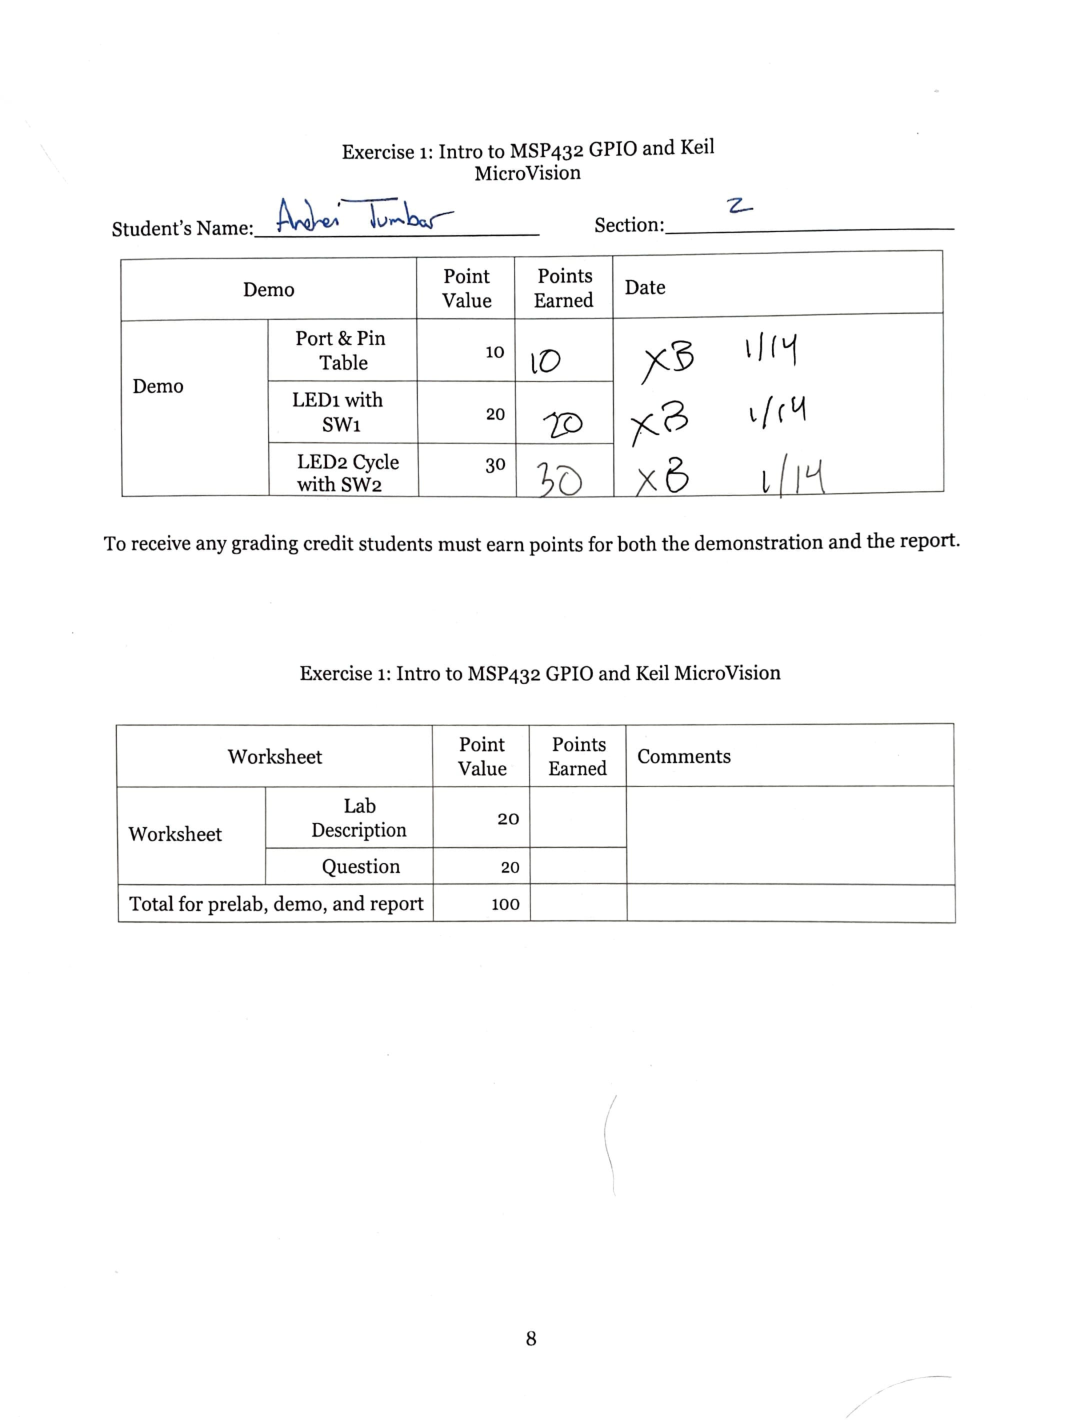
\includepdf[pages=-,pagecommand={},width=\textwidth]{signoff1.pdf}

\end{document}
